\documentclass{beamer}
\usepackage[utf8]{inputenc}

\usetheme{Madrid}
\usecolortheme{default}
\usepackage{extarrows}
\usepackage{amsmath}
\usepackage{extarrows}
\usepackage{amssymb,amsfonts,amsthm}
\usepackage{txfonts}
\usepackage{tkz-euclide}
\usepackage{listings}
\usepackage{adjustbox}
\usepackage{array}
\usepackage{tabularx}
\usepackage{gvv}
\usepackage{lmodern}
\usepackage{circuitikz}
\usepackage{tikz}
\usepackage{graphicx}
\usepackage{amsmath} 

\setbeamertemplate{page number in head/foot}[totalframenumber]

\usepackage{tcolorbox}
\tcbuselibrary{minted,breakable,xparse,skins}

\definecolor{bg}{gray}{0.95}
\DeclareTCBListing{mintedbox}{O{}m!O{}}{%
  breakable=true,
  listing engine=minted,
  listing only,
  minted language=#2,
  minted style=default,
  minted options={%
    linenos,
    gobble=0,
    breaklines=true,
    breakafter=,,
    fontsize=\small,
    numbersep=8pt,
    #1},
  boxsep=0pt,
  left skip=0pt,
  right skip=0pt,
  left=25pt,
  right=0pt,
  top=3pt,
  bottom=3pt,
  arc=5pt,
  leftrule=0pt,
  rightrule=0pt,
  bottomrule=2pt,
  toprule=2pt,
  colback=bg,
  colframe=orange!70,
  enhanced,
  overlay={%
    \begin{tcbclipinterior}
    \fill[orange!20!white] (frame.south west) rectangle ([xshift=20pt]frame.north west);
    \end{tcbclipinterior}},
  #3,
}
\lstset{
    language=C,
    basicstyle=\ttfamily\small,
    keywordstyle=\color{blue},
    stringstyle=\color{orange},
    commentstyle=\color{green!60!black},
    numbers=left,
    numberstyle=\tiny\color{gray},
    breaklines=true,
    showstringspaces=false,
}
\title %optional
{12.46}


\author 
{Kartik Lahoti - EE25BTECH11032}

\begin{document}


\frame{\titlepage}
\begin{frame}{Question}
The eigenvalues of the matrix
\begin{align}
    \vec{P} = \myvec{4 & -5 \\ 2 & -5}
\end{align}
are 
\begin{multicols}
\begin{enumerate}
        \item $-7$ and $8$
        \item $-6$ and $5$
        \item $3$ and $4$
        \item $1$ and $2$
    
\end{enumerate}
\end{multicols}

\end{frame}


\begin{frame}{Theoretical Solution}
\begin{align}
    \mydet{\vec{P} - \lambda\vec{I}} = 0
\end{align}
\begin{align}
    \mydet{\myvec{4-\lambda & -5 \\ 2 & -5-\lambda}} = 0 
\end{align}
\end{frame}
\begin{frame}{Theoretical Solution}
\begin{align}
    \lambda^2 + \lambda -10 = 0
\end{align}
\begin{align}
    \lambda_1 = \frac{-1+\sqrt{41}}{2}, \quad 
    \lambda_2 = \frac{-1-\sqrt{41}}{2}
\end{align}

Hence, Answer : NO CORRECT OPTION
\end{frame}

% \begin{frame}{Plot}
%     \centering
%     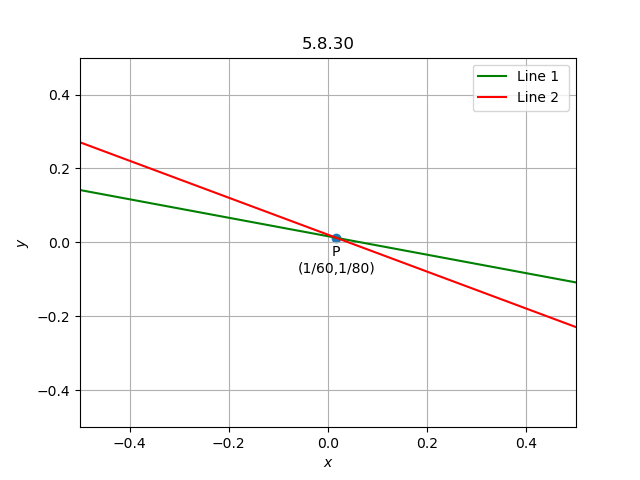
\includegraphics[width=\columnwidth, height=0.8\textheight, keepaspectratio]{../figs/Inter1.png}   
% \end{frame}

\end{document}
